With the intrinsic matrix and distortion coefficients we can undistort images captured with the same camera. The following code is from \texttt{undistort.py}

\subsubsection{Loading parameters}
Just like we saved them, we can load the intrinsic matrix and distortion coefficients with the numpy function \texttt{np.load()}. 

\begin{lstlisting}[language=Python]
mtx = np.load('intrinsic.npy')
dist = np.load('distCoeff.npy')
\end{lstlisting}

\subsubsection{New optimal camera matrix}
This part is optional. By introducing a free scaling parameters alpha, we can control how much of source image pixels are retained. In other words by putting different values for alpha, we control how much black pixels we see at the borders(1 all, 0 none). We create this matrix with \texttt{cv.getOptimalNewCameraMatrix(mtx, dist, (w, h), alpha)}

\begin{lstlisting}[language=Python]
h,  w = img.shape[:2]
alpha = 0
newcameramtx, roi = cv.getOptimalNewCameraMatrix(mtx, dist, (w,h), alpha)
\end{lstlisting}

\subsubsection{Undistort}
To perform the undistortion, we use \texttt{cv.undistort(img, mtx, dist, None, newcameramtx)}

\begin{lstlisting}[language=Python]
dst = cv.undistort(img, mtx, dist, None, newcameramtx)

cv.imshow('dst', dst)
cv.waitKey()
\end{lstlisting}

\begin{figure}[htp]

\centering
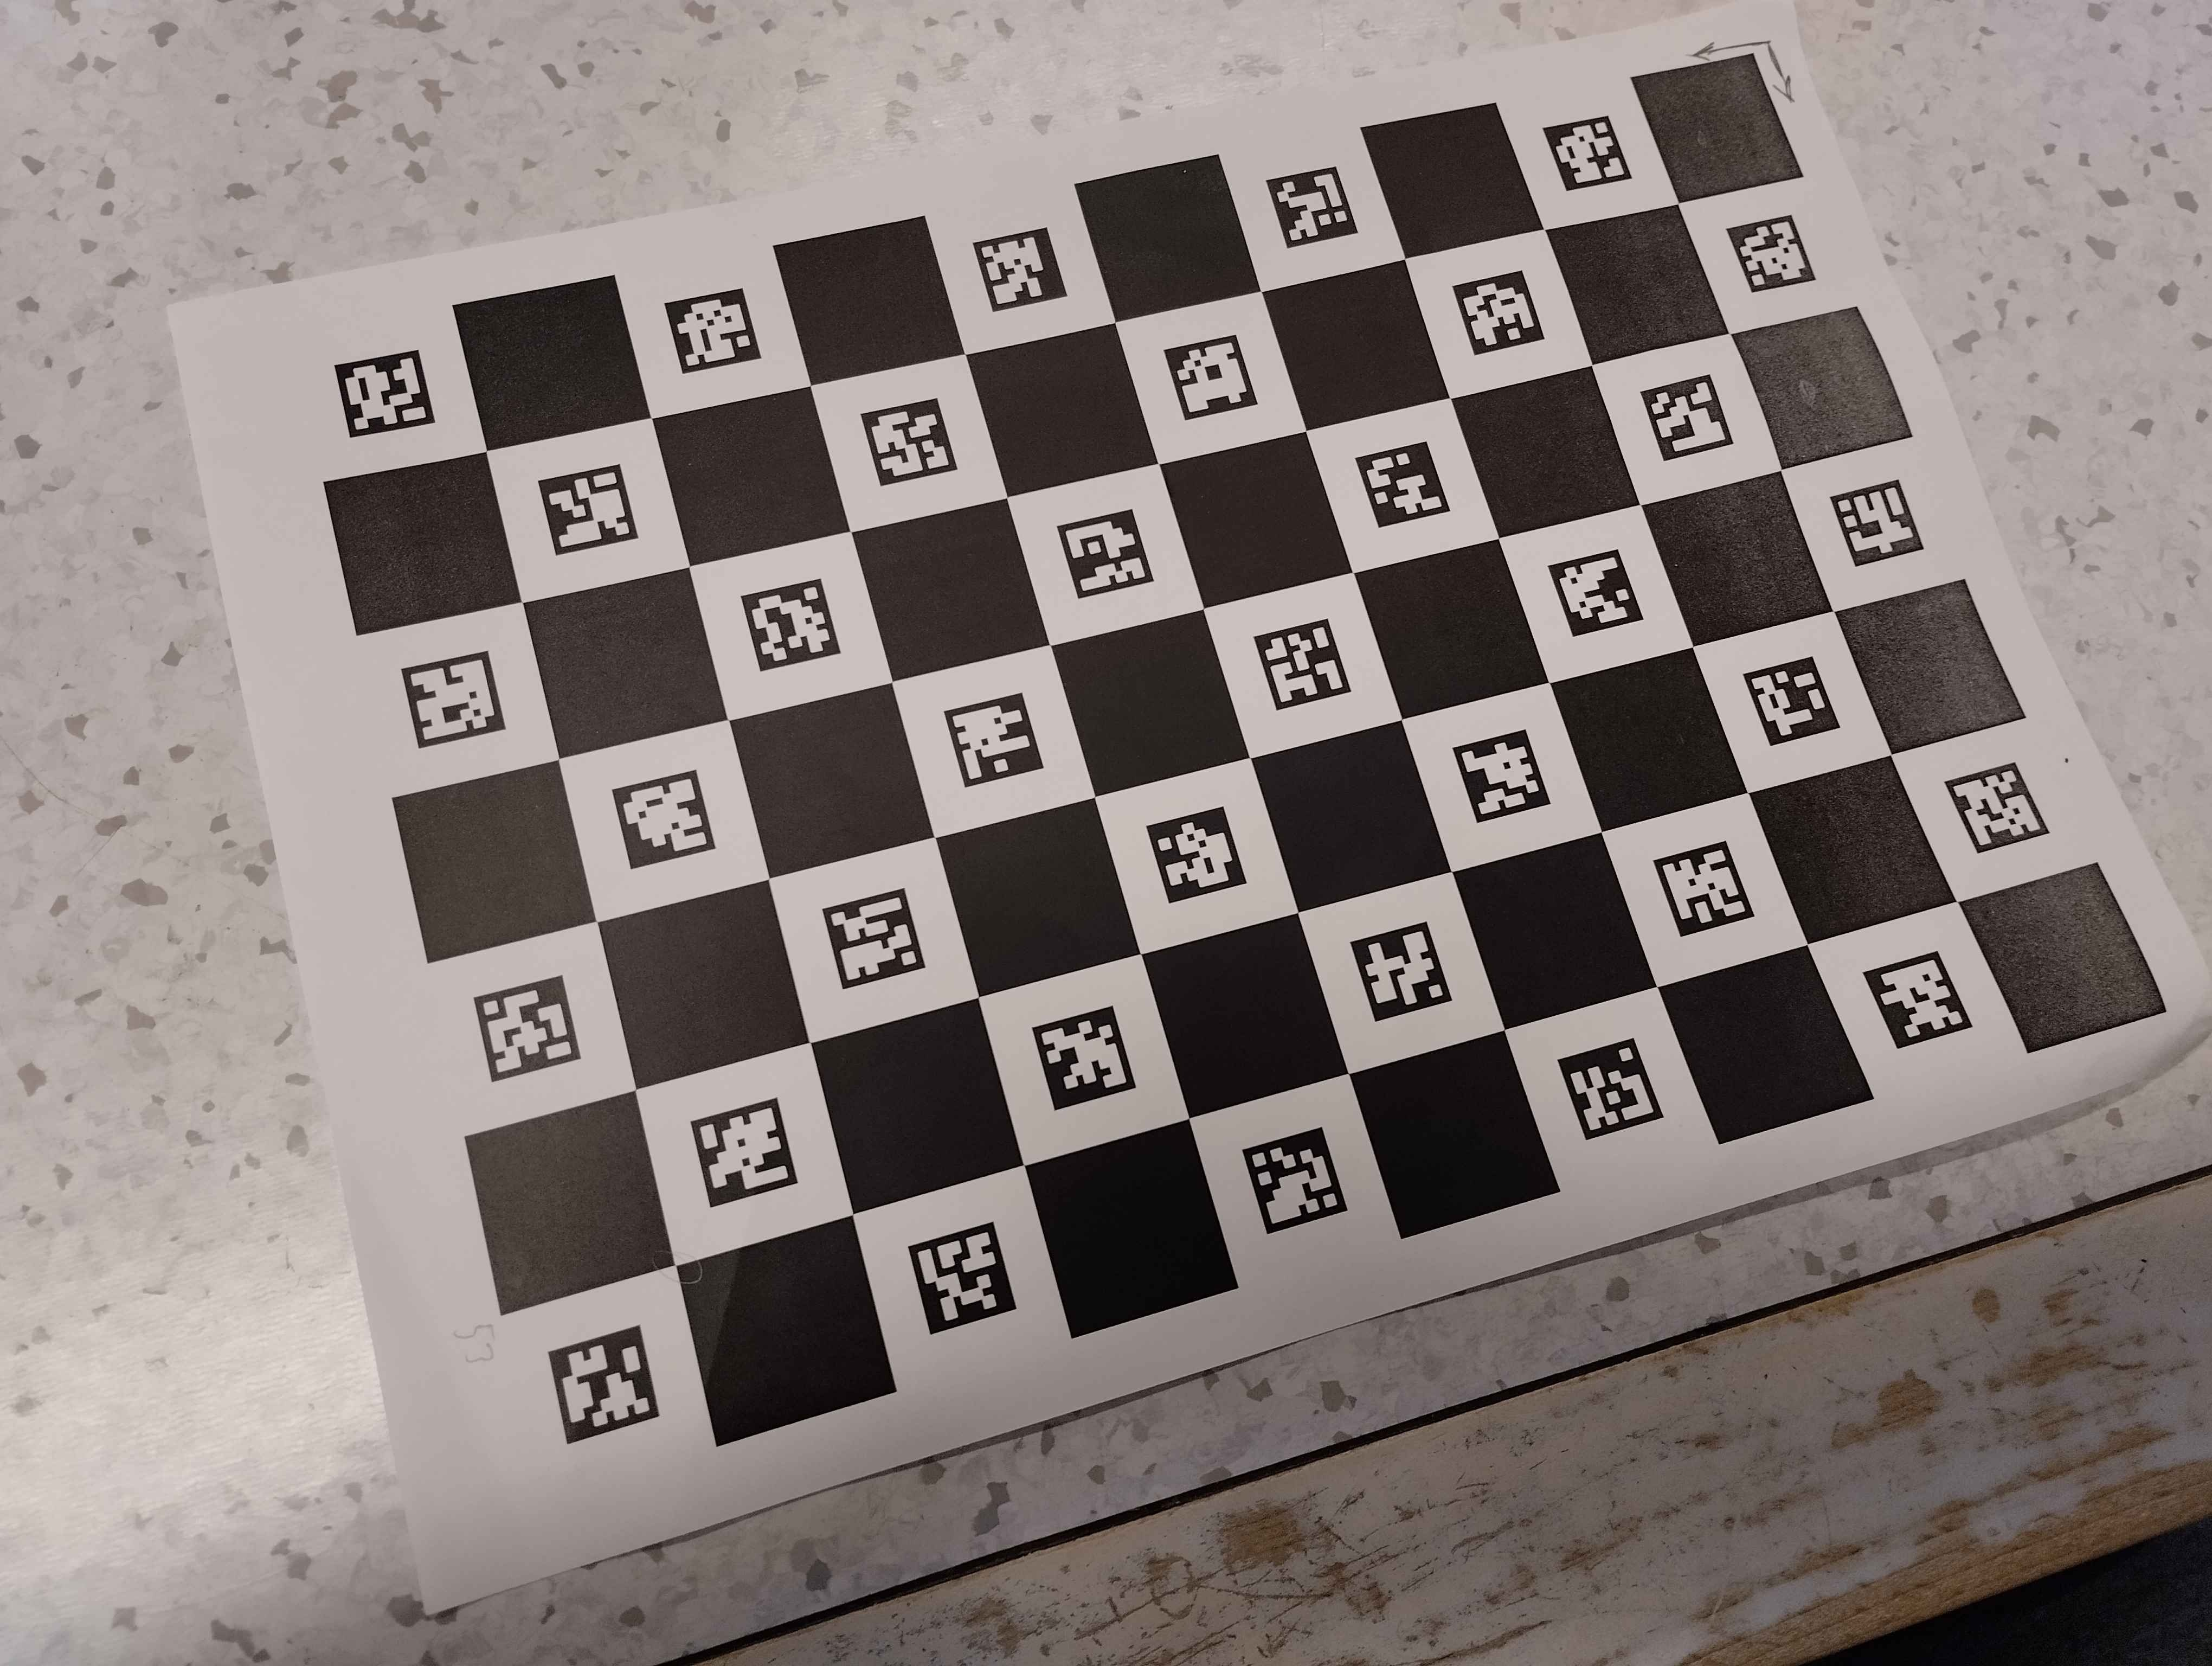
\includegraphics[width=.3\textwidth]{imgs/alphaorg.jpg}\hfill
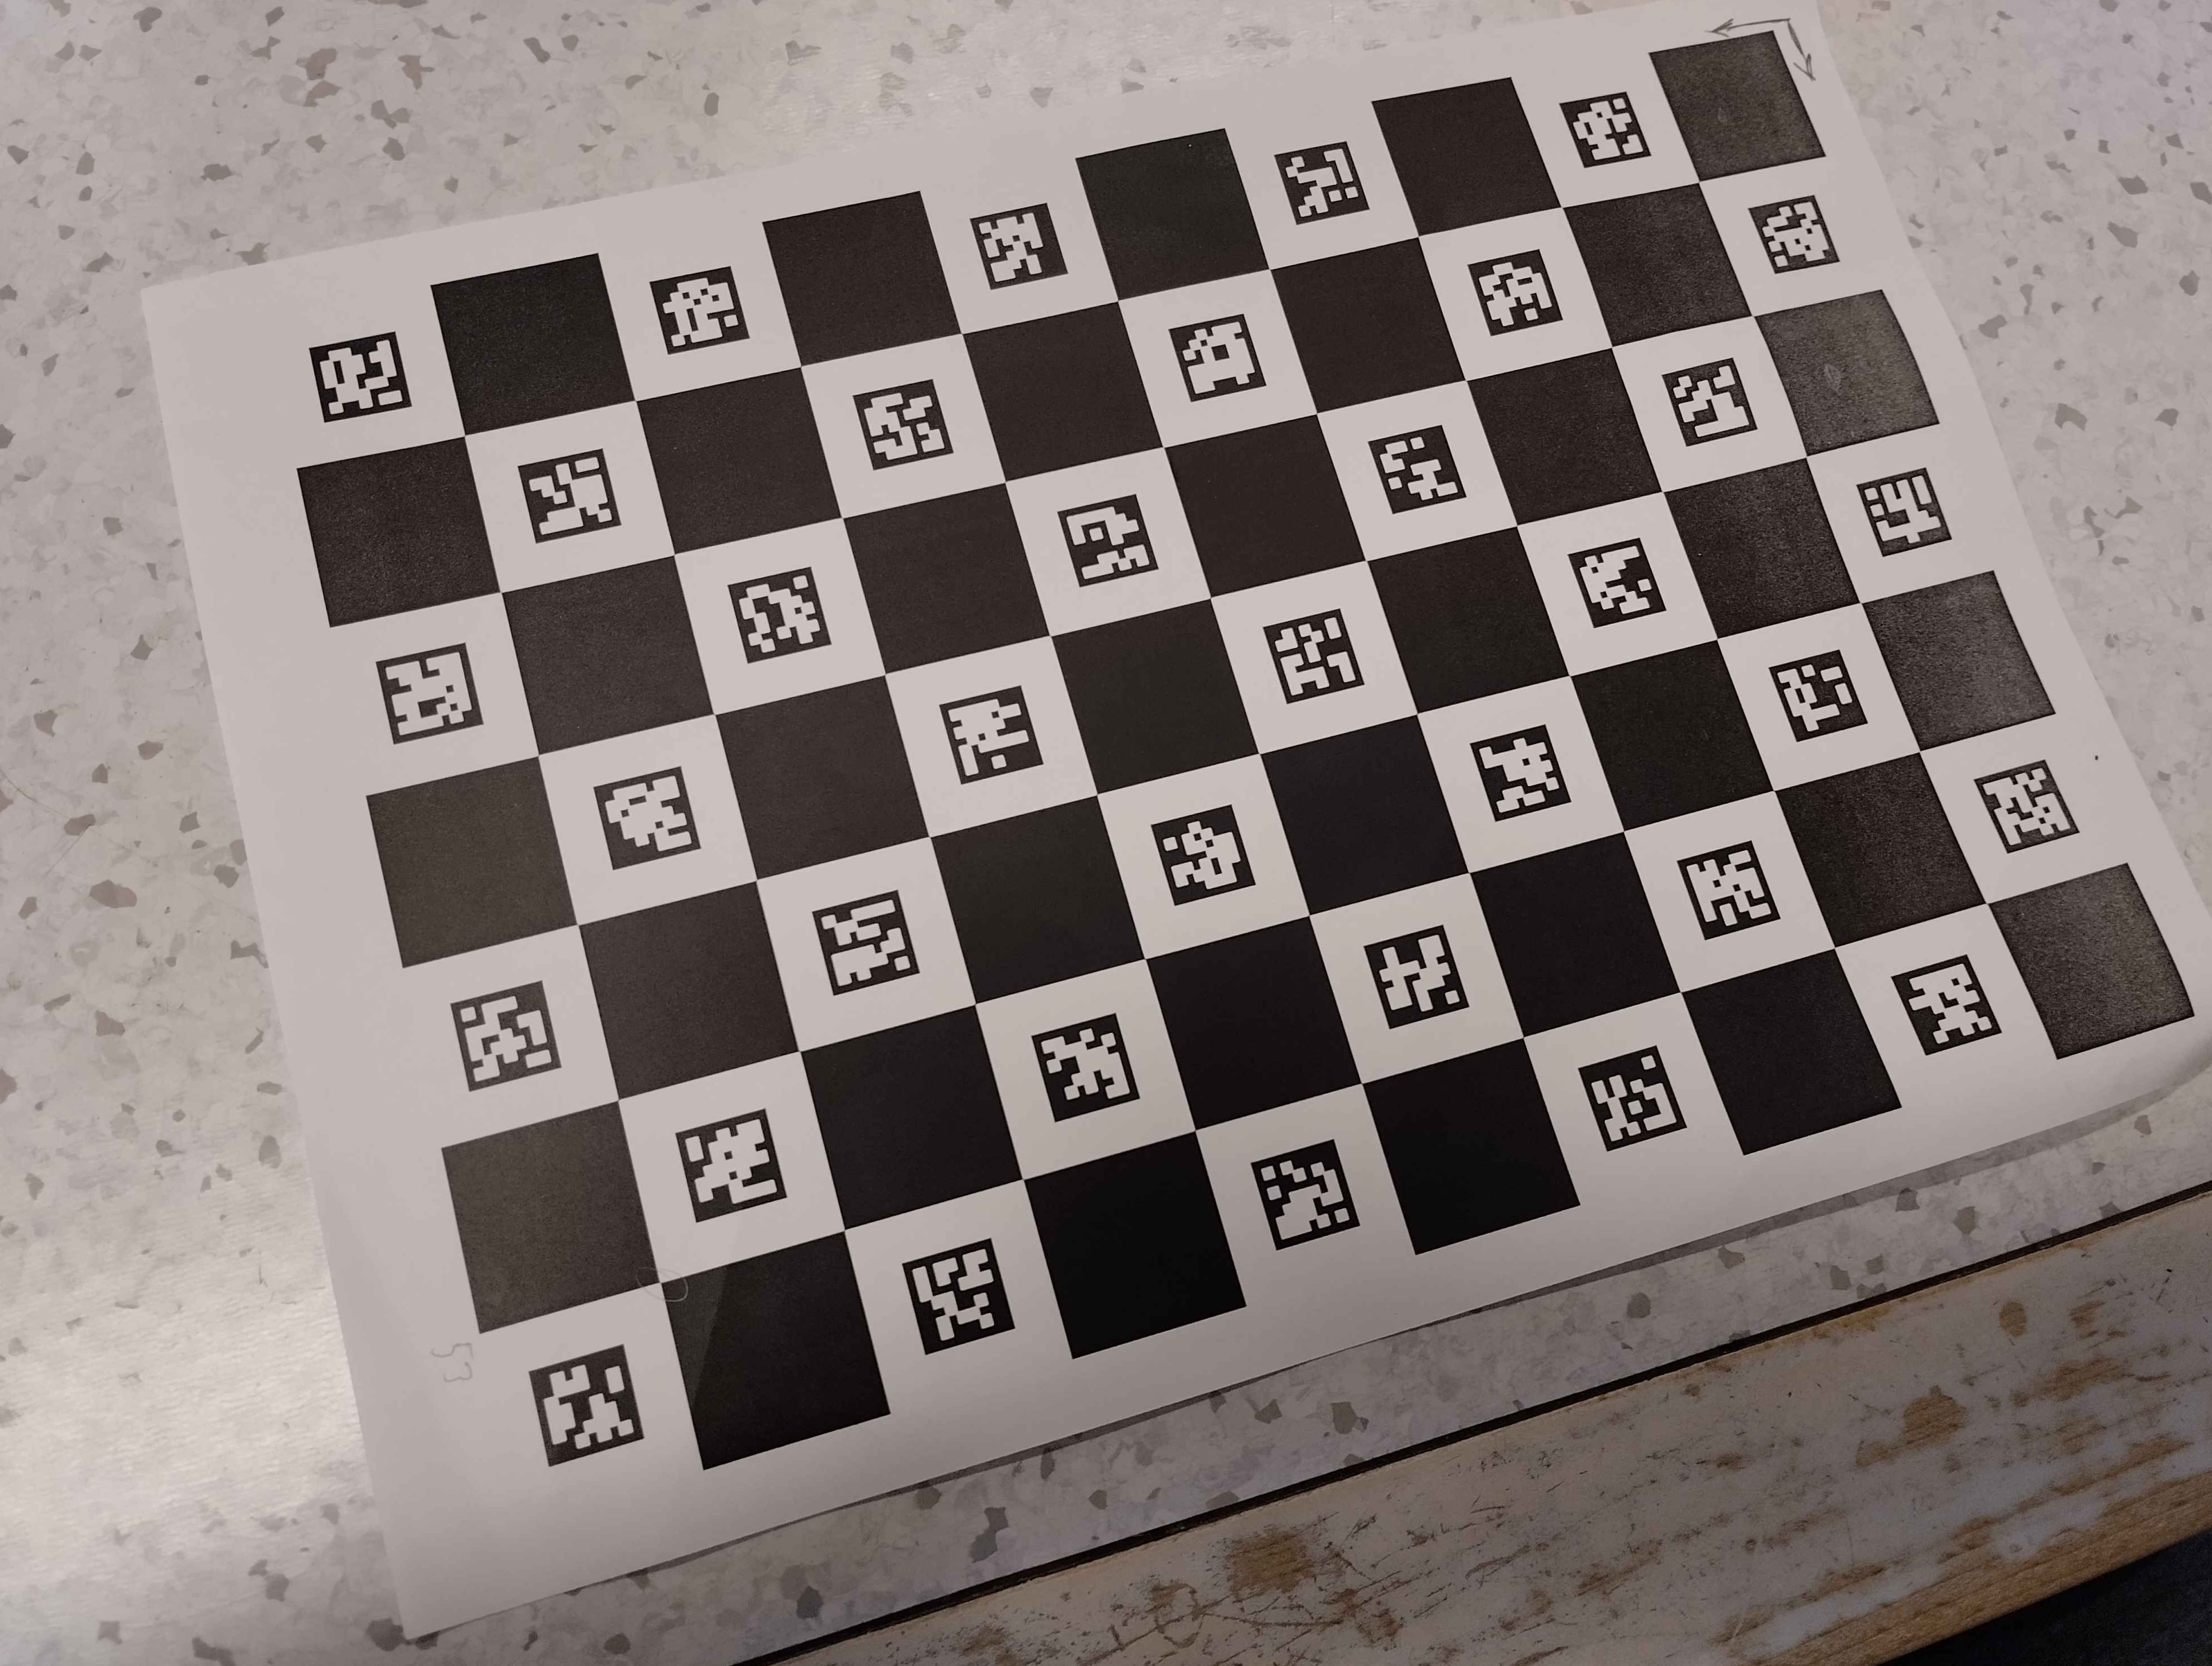
\includegraphics[width=.3\textwidth]{imgs/alpha0.jpg}\hfill
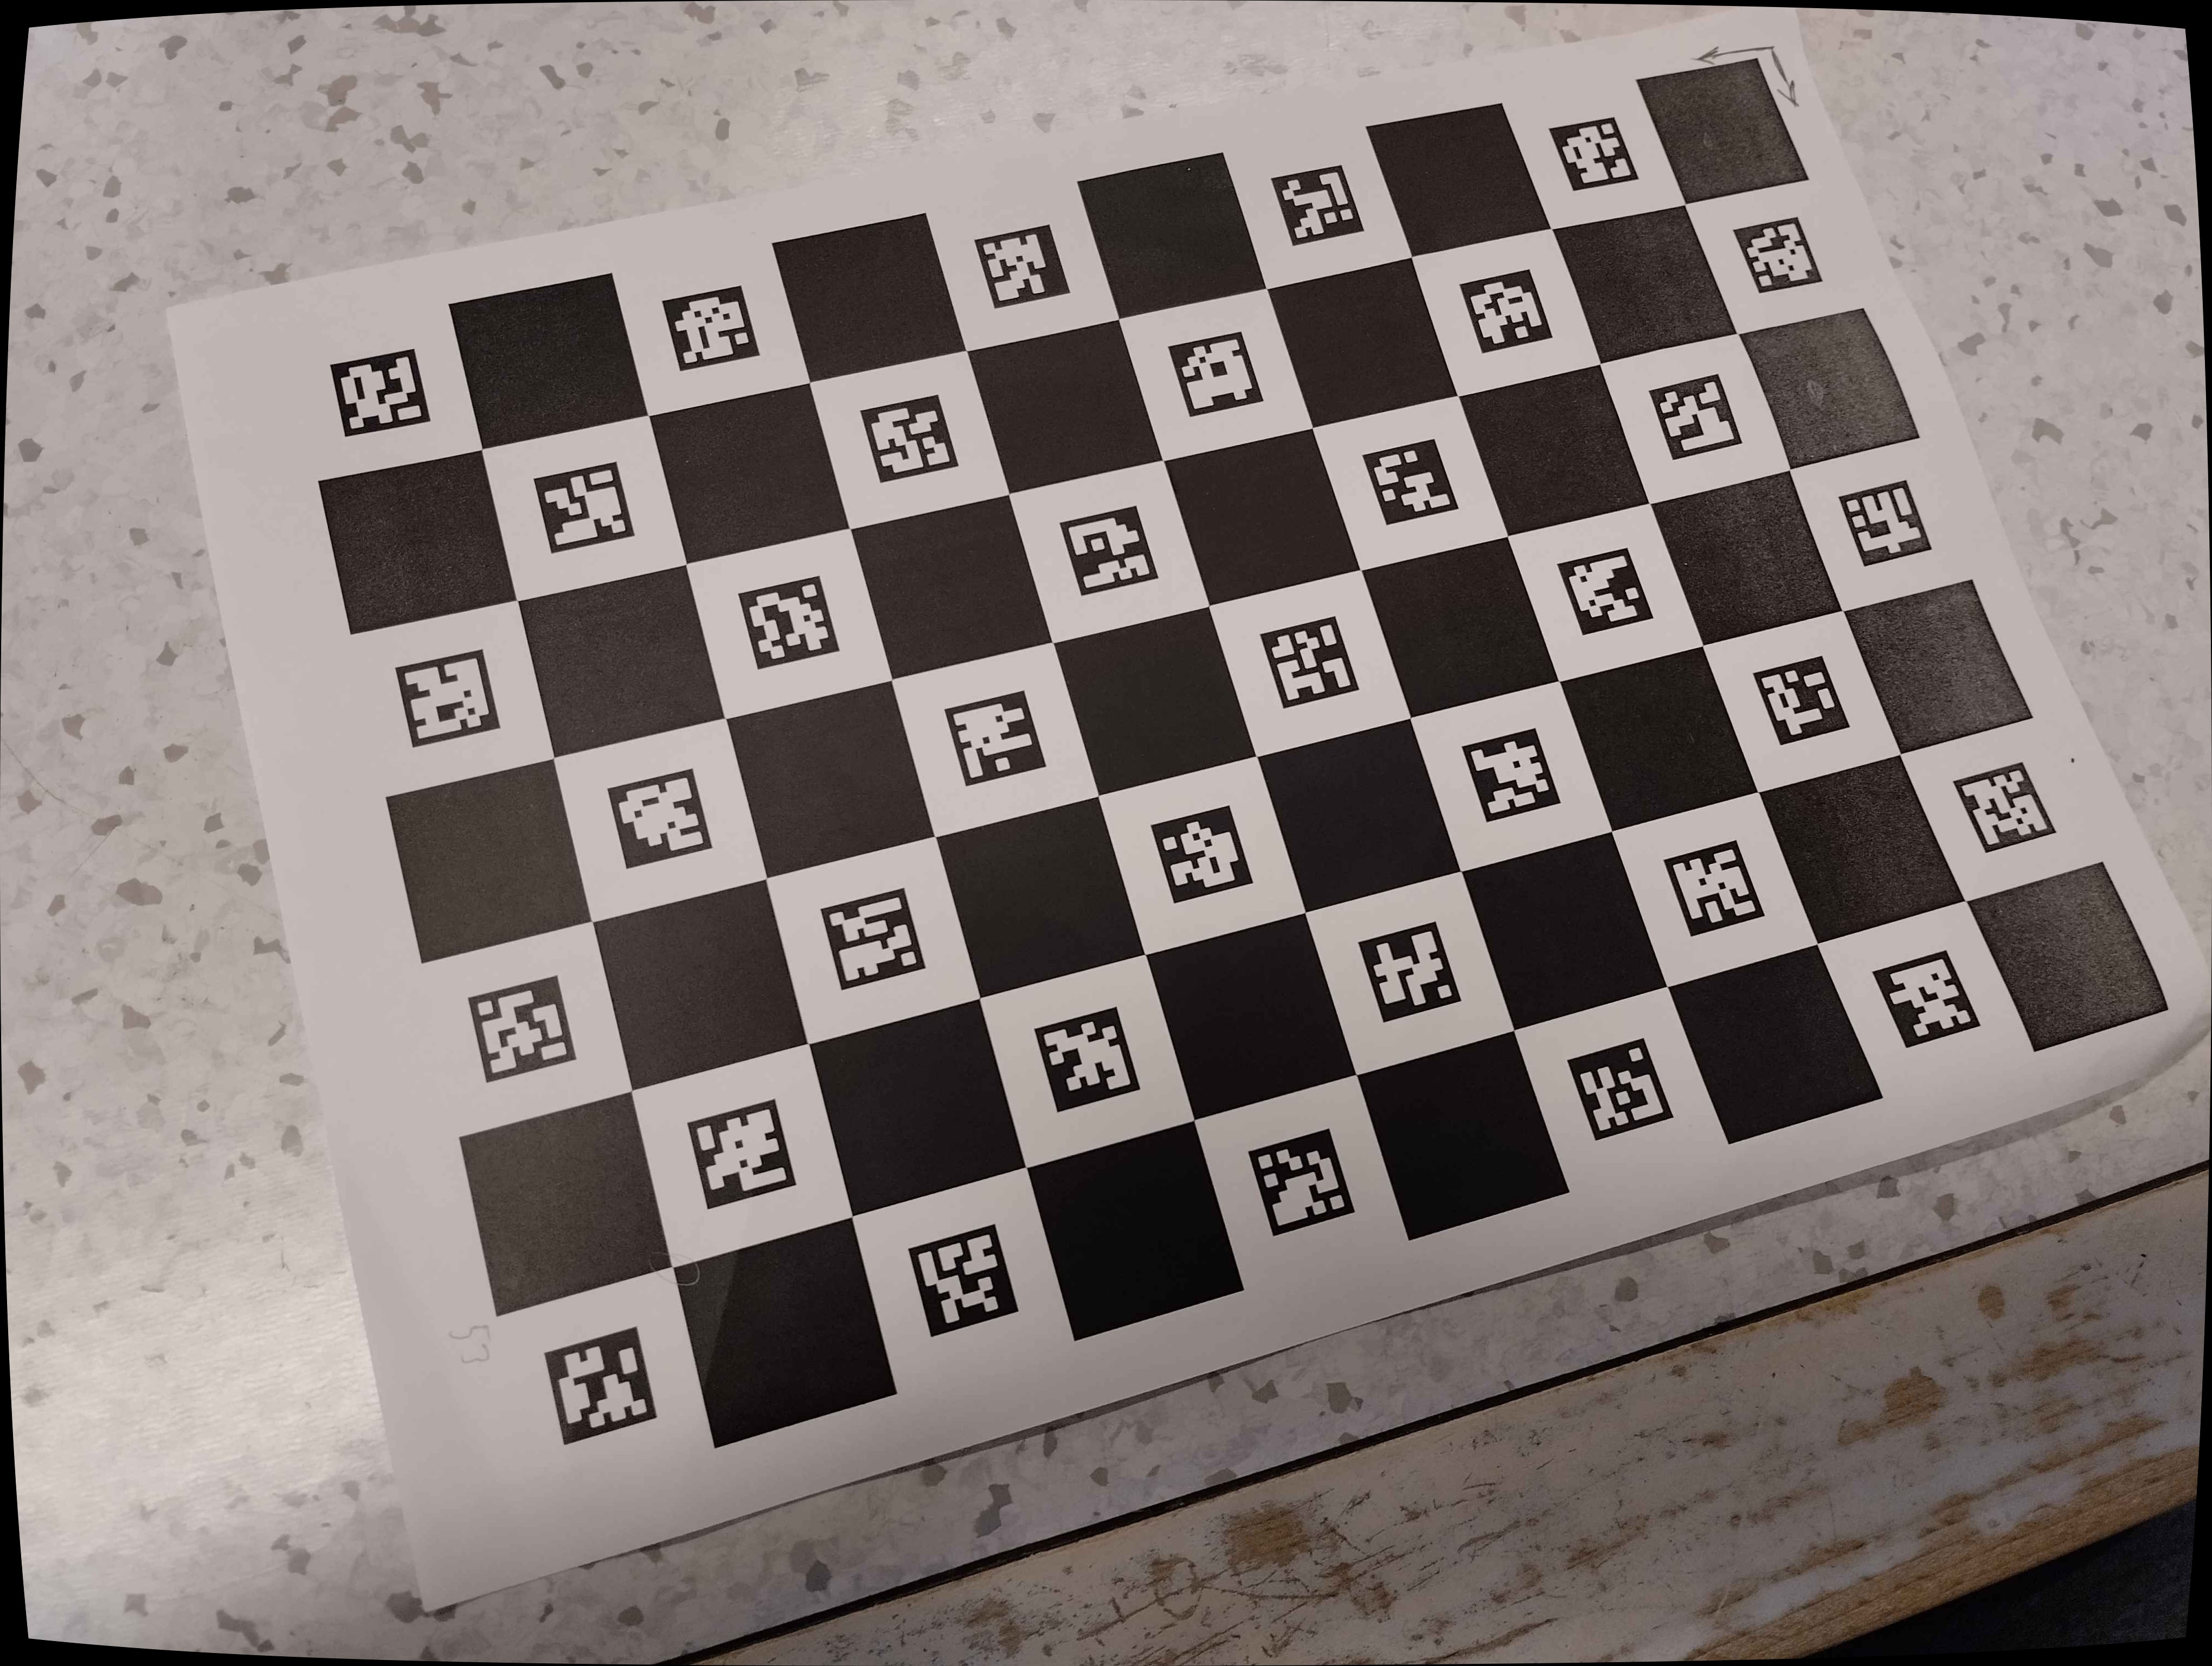
\includegraphics[width=.3\textwidth]{imgs/alpha1.jpg}

\caption{Results: a) original, b) alpha=0, c) alpha=1}
\label{fig:figure3}

\end{figure}